\documentclass[11pt,UTF8]{ctexart}
\usepackage{titling}
\usepackage{enumerate}
\usepackage{amsmath,amssymb,amsfonts}
\usepackage{listings}
\usepackage{comment}
\usepackage{forest}
\usepackage{bm}
\usepackage{float}
\usepackage{graphicx}
\usepackage{multicol,multirow}
\usepackage{bigstrut}
\usepackage[unicode=true,%本行非常重要 支持中文目录hyperref CJKbookmarks对二级目录没用
	colorlinks,
	linkcolor=black,
	anchorcolor=black,
	citecolor=black,
	CJKbookmarks=false]{hyperref}
\usepackage{xcolor}
\usepackage{geometry}
\geometry{top=20mm,bottom=20mm,left=20mm,right=20mm}
\pagestyle{plain}%删除页眉
\CTEXsetup[format={\Large\bfseries}]{section}

\lstset{basicstyle=\small}

\def\toprule{\hline}
\def\midrule{\hline}
\def\bottomrule{\hline}
\newcommand{\ol}[1]{\mathop{\overline{#1}}}%\mathop important!!!

\setlength{\droptitle}{-50pt}%减少标题与页眉距离

\title{数电实验9报告}
\author{17341015\quad数据科学与计算机学院\\计科一班\quad陈鸿峥}
\date{}

\begin{document}
\maketitle
\vspace{-50pt}%减少标题与正文距离
\lstset{language=C++,escapechar=`}

% 真值表 -> 卡诺图 -> 逻辑表达式 -> 选择器件实现
\section{内容一}
\subsection{实验目的}
设计16进制异步加法计数器

\subsection{实验原理}
% Table generated by Excel2LaTeX from sheet 'Sheet1'
\begin{enumerate}
    \item 真值表如下
\begin{table}[H]
  \centering
    \begin{tabular}{|c|c|c|c|r|c|c|c|c|}
\cline{1-4}\cline{6-9}    Q3    & Q2    & Q1    & Q0    &       & Q3    & Q2    & Q1    & Q0 \bigstrut\\
\cline{1-4}\cline{6-9}    0     & 0     & 0     & 0     &       & 1     & 0     & 0     & 0 \bigstrut\\
\cline{1-4}\cline{6-9}    0     & 0     & 0     & 1     &       & 1     & 0     & 0     & 1 \bigstrut\\
\cline{1-4}\cline{6-9}    0     & 0     & 1     & 0     &       & 1     & 0     & 1     & 0 \bigstrut\\
\cline{1-4}\cline{6-9}    0     & 0     & 1     & 1     &       & 1     & 0     & 1     & 1 \bigstrut\\
\cline{1-4}\cline{6-9}    0     & 1     & 0     & 0     &       & 1     & 1     & 0     & 0 \bigstrut\\
\cline{1-4}\cline{6-9}    0     & 1     & 0     & 1     &       & 1     & 1     & 0     & 1 \bigstrut\\
\cline{1-4}\cline{6-9}    0     & 1     & 1     & 0     &       & 1     & 1     & 1     & 0 \bigstrut\\
\cline{1-4}\cline{6-9}    0     & 1     & 1     & 1     &       & 1     & 1     & 1     & 1 \bigstrut\\
\cline{1-4}\cline{6-9}    \end{tabular}%
\end{table}%
    \item 次态卡诺图
    \begin{figure}[H]
        \centering
        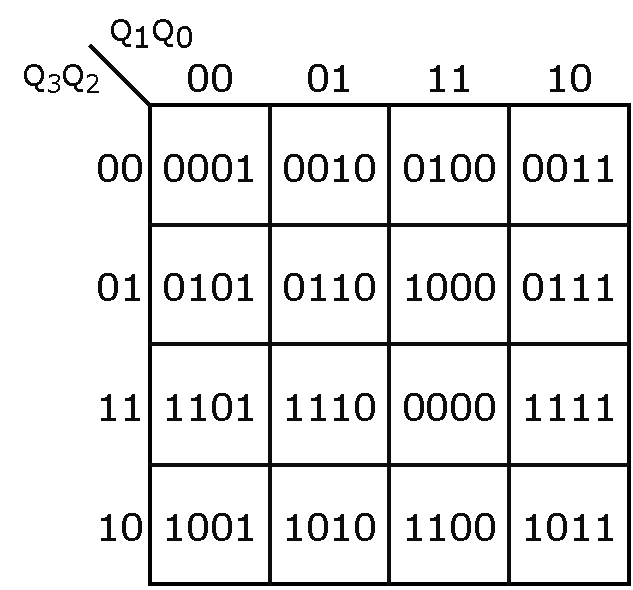
\includegraphics[width=0.4\linewidth]{fig/Karnaugh_additon.pdf}
    \end{figure}
    \item 状态方程
    \[\begin{aligned}
    Q_3^{n+1}&=Q_3\ol{Q_2}+Q_3\ol{Q_1}+Q_3\ol{Q_0}+\ol{Q_3}Q_2Q_1Q_0\\
    Q_2^{n+1}&=Q_2\ol{Q_1}+Q_2\ol{Q_0}+\ol{Q_2}Q_1Q_0\\
    Q_1^{n+1}&=\ol{Q_1}Q_0+Q_1\ol{Q_0}\\
    Q_0^{n+1}&=\ol{Q_0}
    \end{aligned}\]
    \item 驱动方程,将状态方程化为JK触发器形式可得
    \[\begin{aligned}
    J_0&=1 \qquad &K_0&=1\\
    J_1&=Q_0 \qquad &K_0&=Q_0\\
    J_2&=Q_1Q_0 \qquad &K_2&=Q_1Q_0\\
    J_3&=Q_2Q_1Q_0 \qquad &K_3&=Q_2Q_1Q_0
    \end{aligned}\]
\end{enumerate}

\subsection{实验细节}
\subsubsection{Protues仿真}
\par 电路图如下所示
\begin{figure}[H]
    \centering
    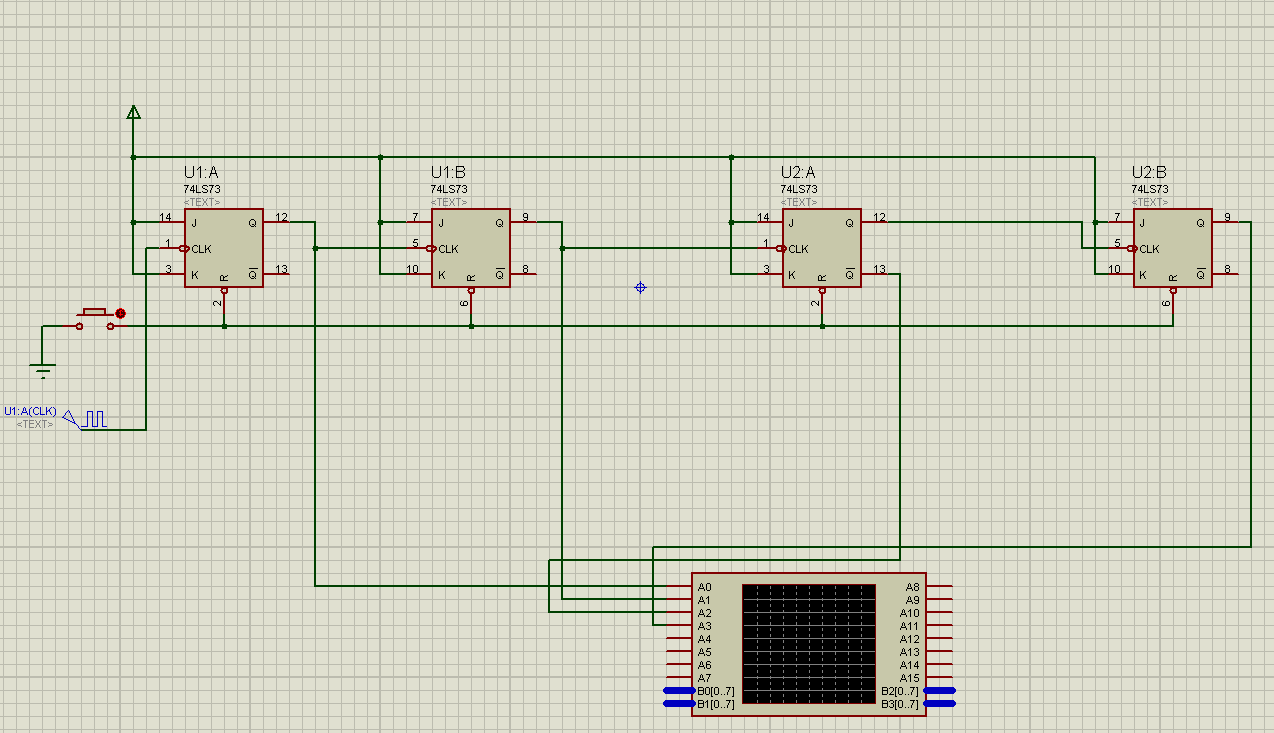
\includegraphics[width=0.8\linewidth]{fig/16addition_asyn.PNG}
\end{figure}
\par 仿真结果如下
\begin{figure}[H]
    \centering
    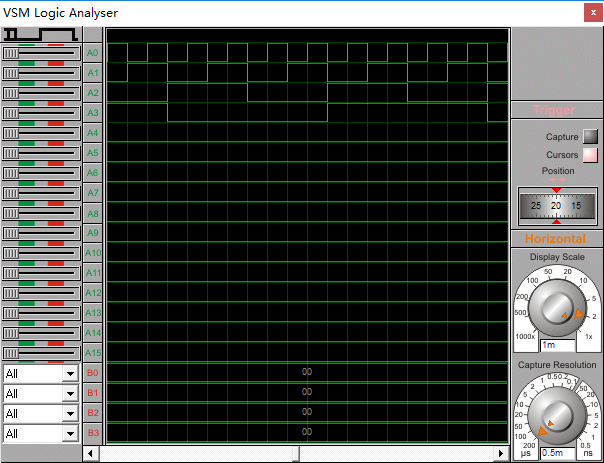
\includegraphics[width=0.6\linewidth]{fig/16addition_asyn_wave.PNG}
\end{figure}

\subsubsection{实验仪器及器件}
\begin{enumerate}
    \item 数字电路实验箱、示波器、导线若干
    \item 74LS73*4
\end{enumerate}

\subsubsection{实验流程与结果分析}
\par 如Protues电路连线
\par 实验箱连线如下
\begin{figure}[H]
    \centering
    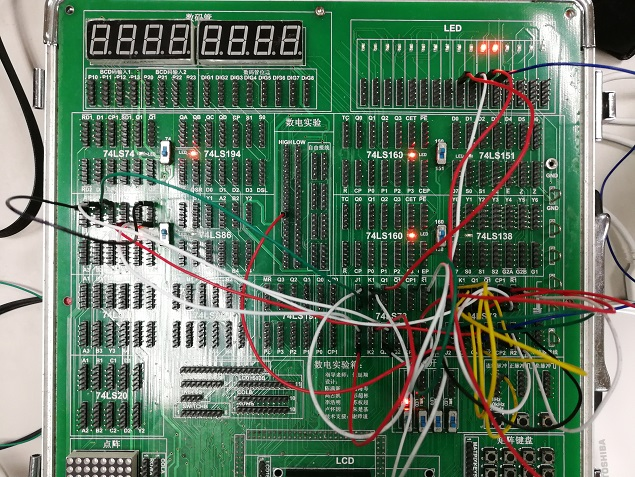
\includegraphics[width=0.6\linewidth]{fig/adder_1.jpg}
\end{figure}
\par 通过观察01显示器,符合波形


\section{内容二}
\subsection{实验目的}
实现16进制同步加法计数器

\subsection{实验原理}
\par 同实验1

\subsection{实验细节}
\subsubsection{Protues仿真}
\par 电路图如下所示
\begin{figure}[H]
    \centering
    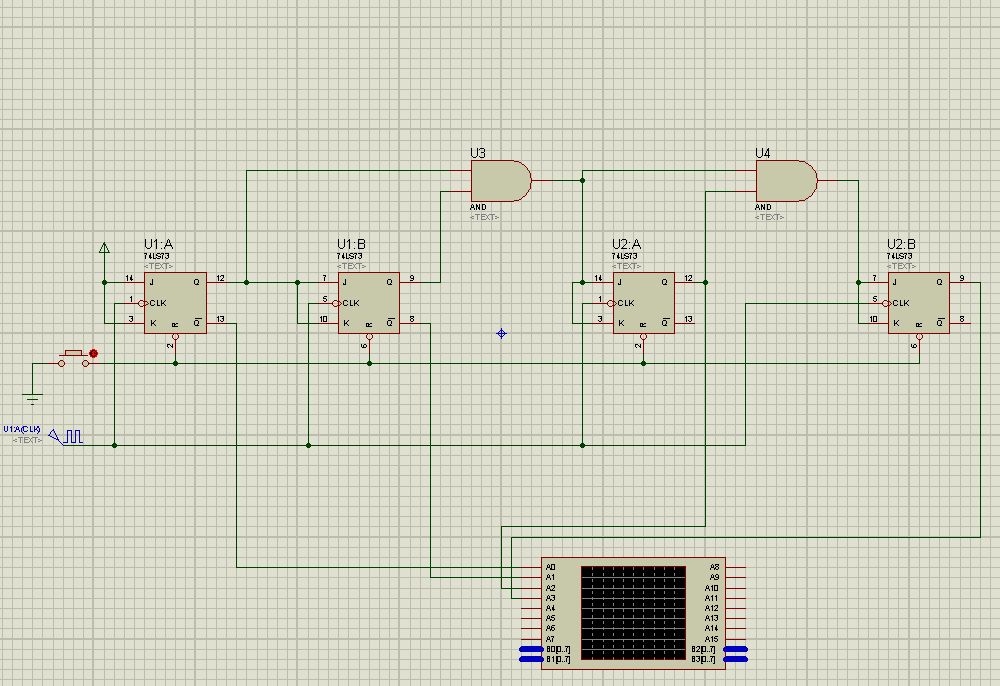
\includegraphics[width=0.8\linewidth]{fig/16addition_syn.PNG}
\end{figure}
\par 仿真结果如下
\begin{figure}[H]
    \centering
    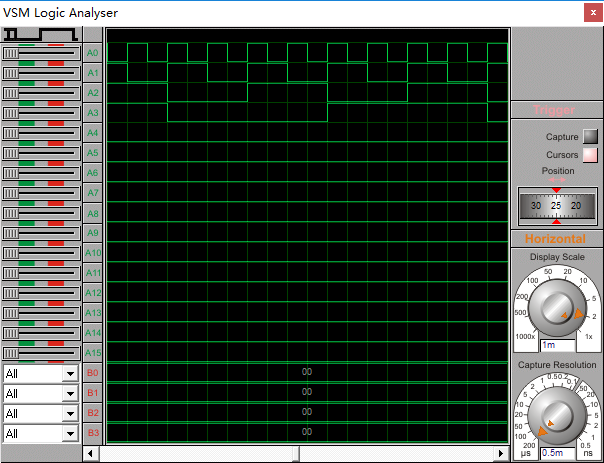
\includegraphics[width=0.6\linewidth]{fig/16addition_syn_wave.PNG}
\end{figure}

\subsubsection{实验仪器及器件}
\begin{enumerate}
    \item 数字电路实验箱、示波器、导线若干
    \item 74LS73*4
\end{enumerate}

\subsubsection{实验流程及结果分析}
\par 如Protues电路连线
\par 实验箱连线如下
\begin{figure}[H]
    \centering
    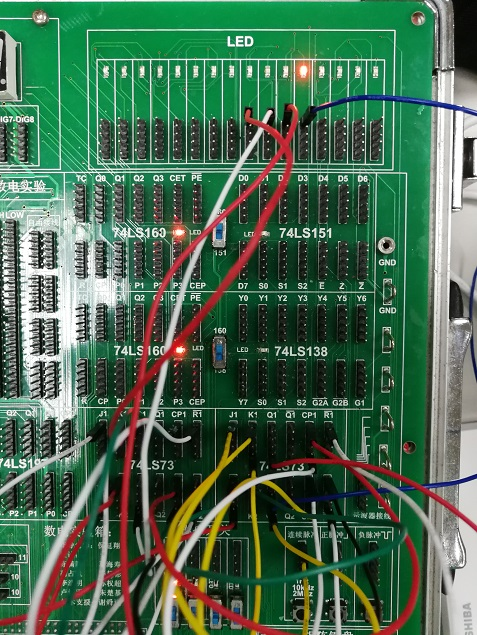
\includegraphics[width=0.6\linewidth]{fig/adder_2.jpg}
\end{figure}
\par 通过观察01显示器,符合波形



\section{内容三}
\subsection{实验目的}
使用JK触发器和门电路设计实现一个二进制四位计数器模仿74LS194功能

\subsection{实验原理}
\par 74LS194功能如下
\begin{table}[H]
  \centering
    \begin{tabular}{|c|c|c|c|}
    \hline
    $\overline{Cr}$    & $S_1$    & $S_0$ & 功能 \bigstrut\\
    \hline
    0     & X & X     & 置零 \bigstrut\\
    \hline
    1     & 0 & 0     & 保持 \bigstrut\\
    \hline
    1     & 0 & 1     & 右移 \bigstrut\\
    \hline
    1     & 1 & 0     & 左移 \bigstrut\\
    \hline
    1 & 1 & 1 & 并行送数\\
    \hline
    \end{tabular}%
\end{table}%
\par 仅左移右移次态卡诺图
\begin{figure}[H]
    \centering
    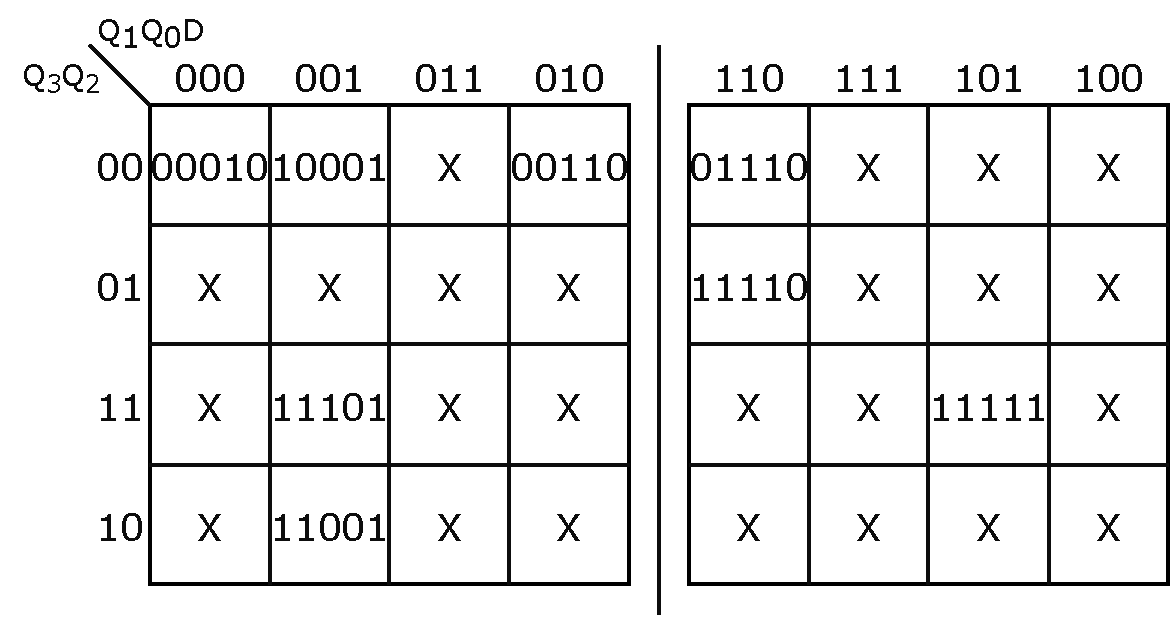
\includegraphics[width=0.6\linewidth]{fig/ls_and_rs.pdf}
\end{figure}
\par 状态方程
    \[\begin{aligned}
    Q_3^{n+1}&=Q_2+D\\
    Q_2^{n+1}&=Q_3+Q_1\\
    Q_1^{n+1}&=Q_2+Q_1+Q_0\\
    Q_0^{n+1}&=Q_1+\ol{D}
    \end{aligned}\]
\par 驱动方程,将状态方程化为JK触发器形式可得
    \[\begin{aligned}
    J_0&=\ol{\ol{Q_1}D} \qquad &K_0&=\ol{Q_1}D\\
    J_1&=\ol{\ol{Q_2}\ol{Q_0}} \qquad &K_0&=0\\
    J_2&=\ol{\ol{Q_3}\ol{Q_1}} \qquad &K_2&=\ol{Q_3}\ol{Q_1}\\
    J_3&=\ol{\ol{Q_2}\ol{D}} \qquad &K_3&=\ol{Q_2}\ol{D}
    \end{aligned}\]

\subsection{实验细节}
\subsubsection{Protues仿真}
\par 全功能74LS194电路图如下
\begin{figure}[H]
    \centering
    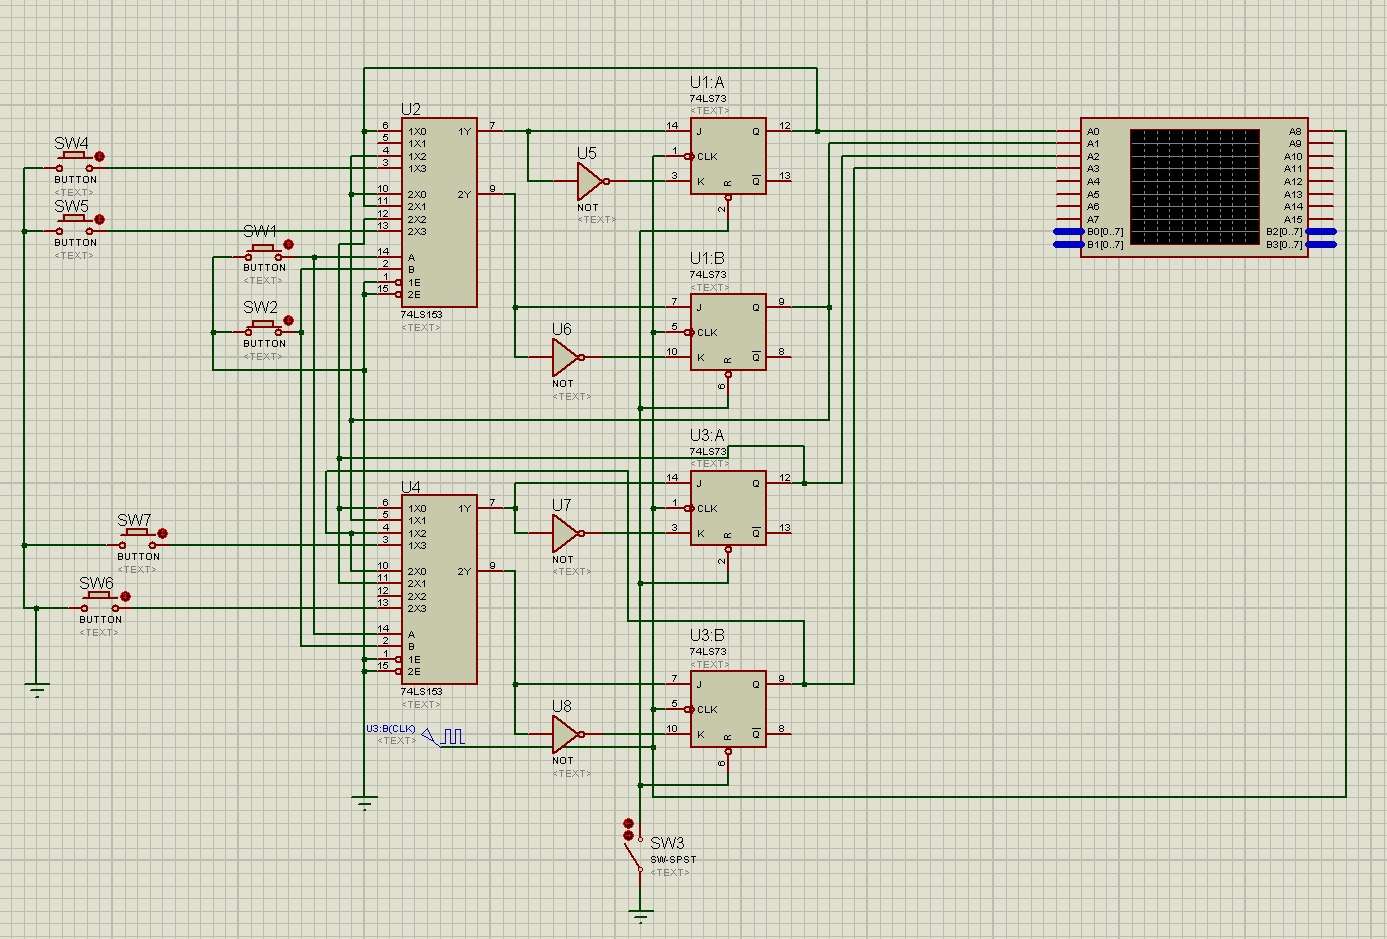
\includegraphics[width=0.6\linewidth]{fig/74ls194.PNG}
\end{figure}
\par 具体功能测试如下
\begin{enumerate}
\item 左移
\begin{figure}[H]
    \centering
    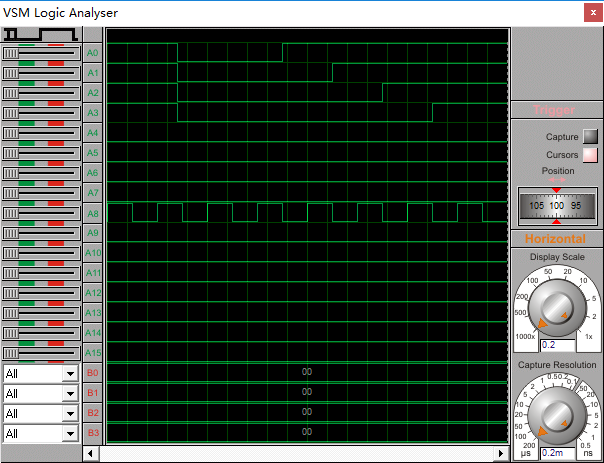
\includegraphics[width=0.6\linewidth]{fig/ls.PNG}
\end{figure}
\item 右移
\begin{figure}[H]
    \centering
    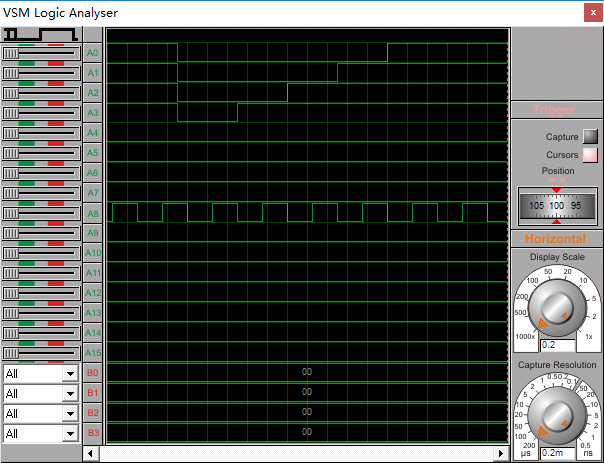
\includegraphics[width=0.6\linewidth]{fig/rs.PNG}
\end{figure}
\item 并行送数,图为1011
\begin{figure}[H]
    \centering
    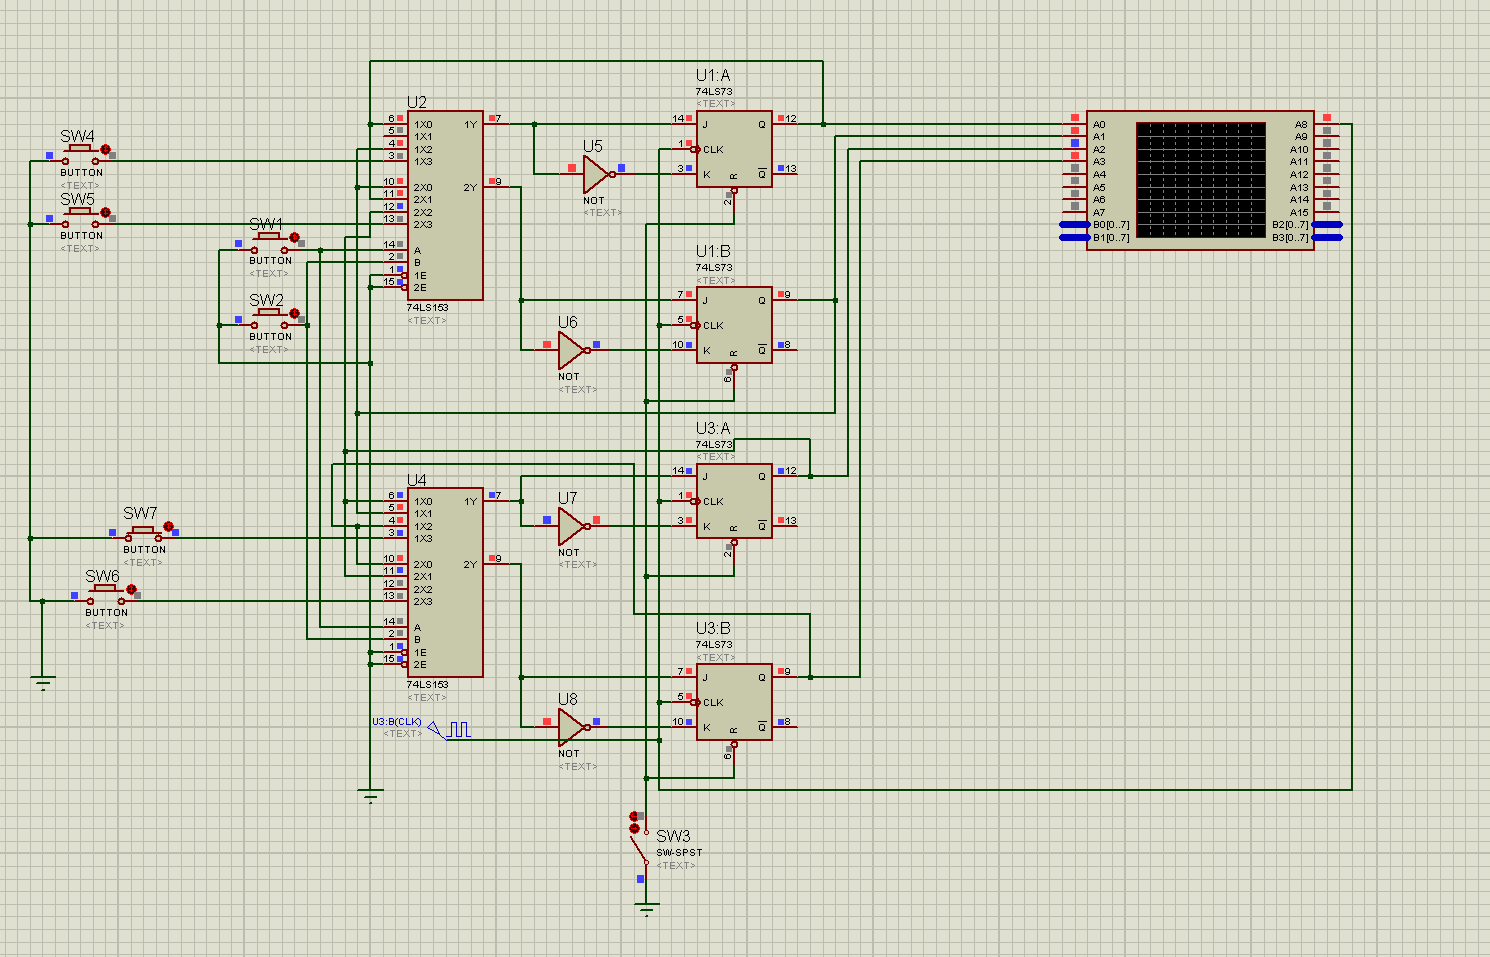
\includegraphics[width=0.6\linewidth]{fig/parallel.PNG}
\end{figure}
\item 保持,图为左移过程中出现0011后立即切换状态为保持
\begin{figure}[H]
    \centering
    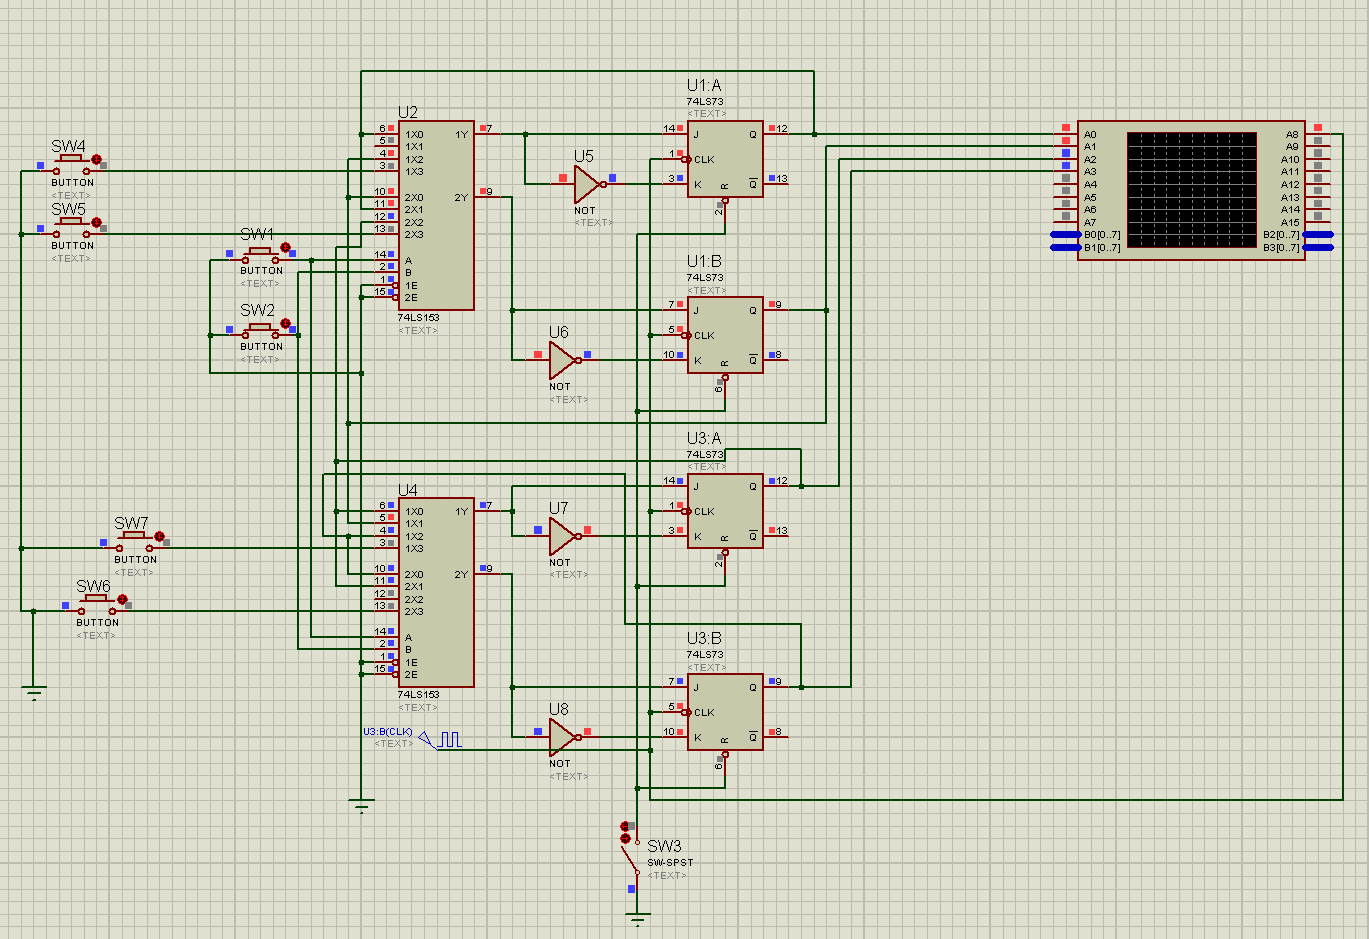
\includegraphics[width=0.6\linewidth]{fig/hold.PNG}
\end{figure}
\end{enumerate}
\par 仅左移右移74LS194电路图如下
\begin{figure}[H]
    \centering
    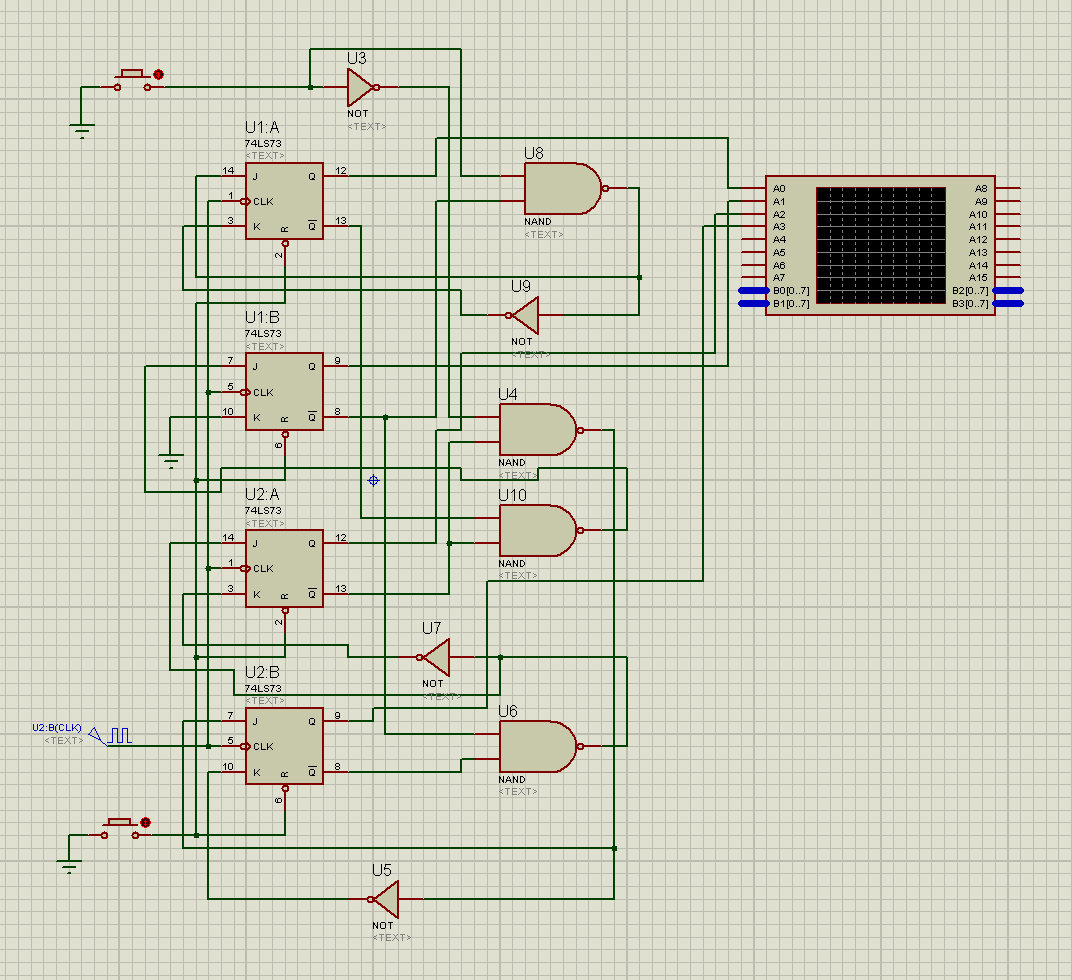
\includegraphics[width=0.6\linewidth]{fig/lsrs_circuit.PNG}
\end{figure}

\subsubsection{实验仪器及器件}
\begin{enumerate}
    \item 数字电路实验箱、示波器、导线若干
    \item 74LS73*4
\end{enumerate}

\subsubsection{实验流程与结果分析}
\par 连线如Protues所示,结果如下图
\begin{figure}[H]
    \centering
    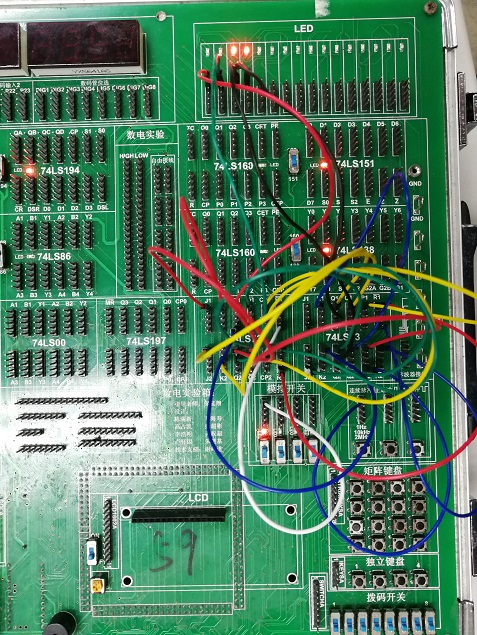
\includegraphics[width=0.6\linewidth]{fig/lsrs.jpg}
\end{figure}



\section{内容四}
\subsection{实验目的}
用JK触发器实现12进制同步计数器

\subsection{实验原理}
\begin{enumerate}
    \item 状态转换图
    \begin{figure}[H]
        \centering
        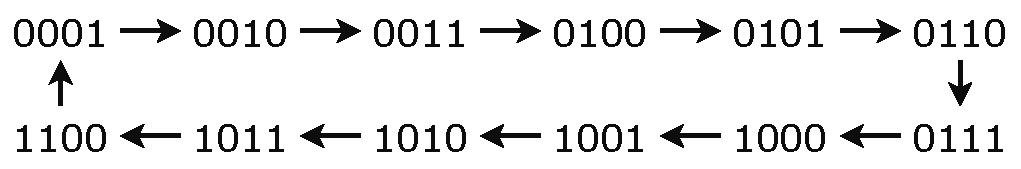
\includegraphics[width=0.7\linewidth]{fig/12system_state.pdf}
    \end{figure}
    \item 确定电路所需触发器数目\\
    由于$2^4=16>12$,故需要$4$个JK触发器
    \item 次态卡诺图
    \begin{figure}[H]
        \centering
        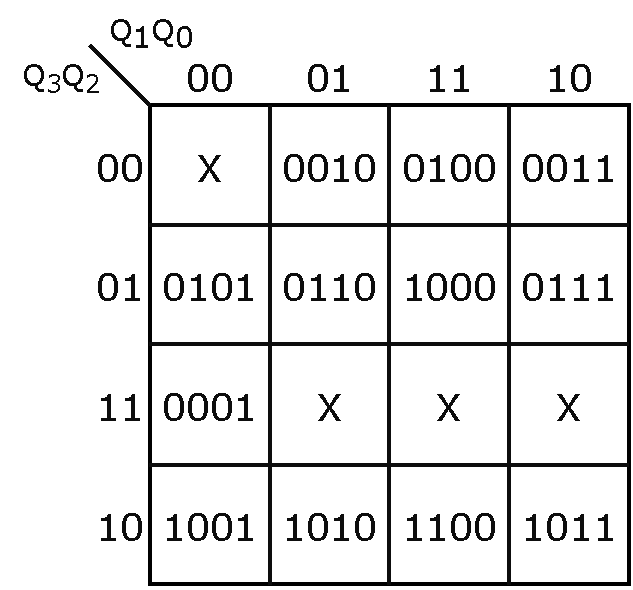
\includegraphics[width=0.4\linewidth]{fig/Karnaugh_12system.pdf}
    \end{figure}
    \item 触发器状态方程,由卡诺图可得
    \[\begin{aligned}
    Q_0^{n+1}&=\overline{Q_0}\\
    Q_1^{n+1}&=Q_0\overline{Q_1}+\overline{Q_0}Q_1\\
    Q_2^{n+1}&=Q_0Q_1\ol{Q_2}+\ol{Q_1}Q_2\ol{Q_3}+\ol{Q_0}Q_2\ol{Q_3}\\
    Q_3^{n+1}&=\ol{Q_2}Q_3+Q_0Q_1Q_2\ol{Q_3}
    \end{aligned}\]
    \item 触发器驱动方程,由
    \[Q^{n+1}=J\ol{Q^n}+\ol{K}Q^n\]
    将状态方程整理为上式形式,可得
    \[\begin{aligned}
    J_0&=1 \qquad &K_0&=1\\
    J_1&=Q_0 \qquad &K_0&=Q_0\\
    J_2&=Q_1Q_0 \qquad &K_2&=\ol{\ol{Q_3}\ol{Q_1}+\ol{Q_3}\ol{Q_0}}=\ol{Q_3}+Q_1Q_0\\
    J_3&=Q_2Q_1Q_0 \qquad &K_3&=Q_2
    \end{aligned}\]
    \item 检查自启动\\
    当输入为1111和0000时,可自动跳转至0001;输入为1101时,跳转至0010;输入为1110时,跳转至0011
\end{enumerate}

\subsection{Protues仿真}
\par 电路图连接如下
\begin{figure}[H]
    \centering
    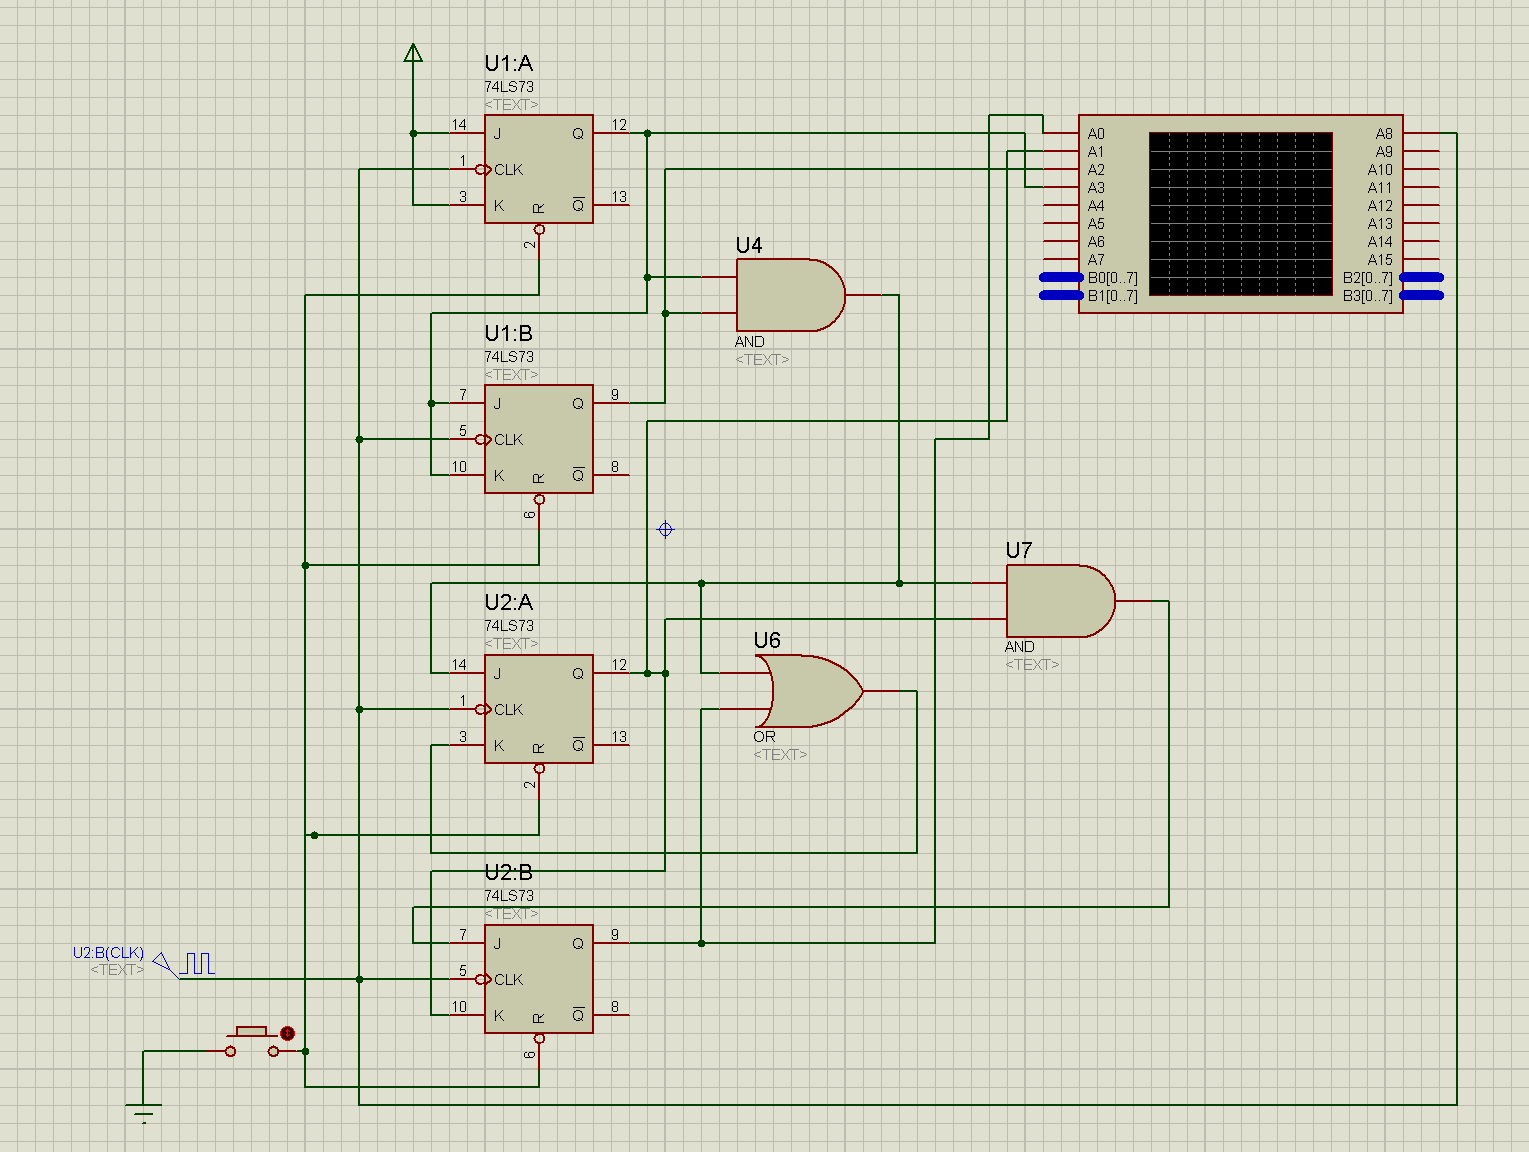
\includegraphics[width=0.9\linewidth]{fig/12system_protues.PNG}
\end{figure}
\par 仿真结果如下
\begin{figure}[H]
    \centering
    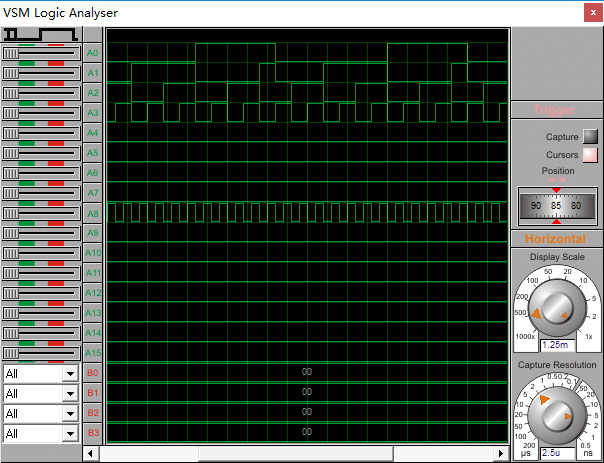
\includegraphics[width=0.6\linewidth]{fig/12system_wave.PNG}
\end{figure}
\par 波形符合12进制转换

\subsection{实验细节}
\subsubsection{实验仪器及器件}
\begin{enumerate}
    \item 数字电路实验箱、示波器、导线若干
    \item 74LS73*4,74LS00*2,74LS08*2
\end{enumerate}

\subsubsection{实验流程与结果分析}
\par 如Protues电路图所示连线
\par 将输出接01显示器,可见01显示器按照状态转换图顺序依次闪烁
\begin{figure}[H]
    \centering
    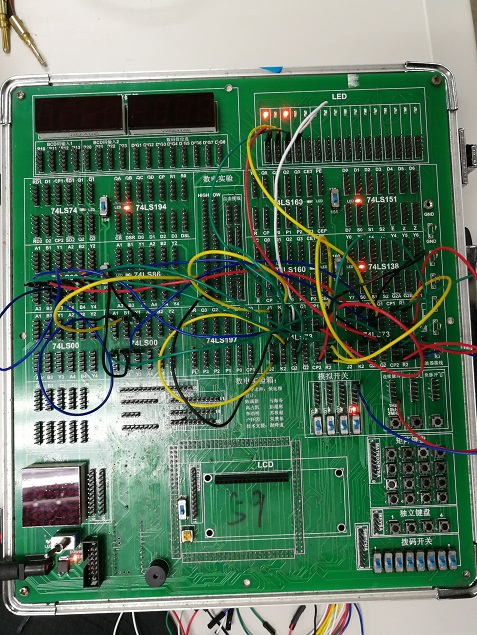
\includegraphics[width=0.6\linewidth]{fig/broad_12system.jpg}
\end{figure}



\section{内容五}
\subsection{实验目的}
用Protues和Vivado分别实现一个有控制变量D的12进制计数器,并在七段数码管上显示计数结果

\subsection{实验原理}
\begin{enumerate}
    \item 状态转移图
    \begin{figure}[H]
        \centering
        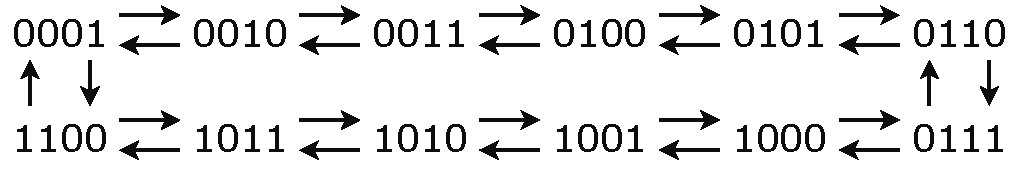
\includegraphics[width=0.6\linewidth]{fig/12system_2.pdf}
    \end{figure}
    \item 次态卡诺图
    \begin{figure}[H]
        \centering
        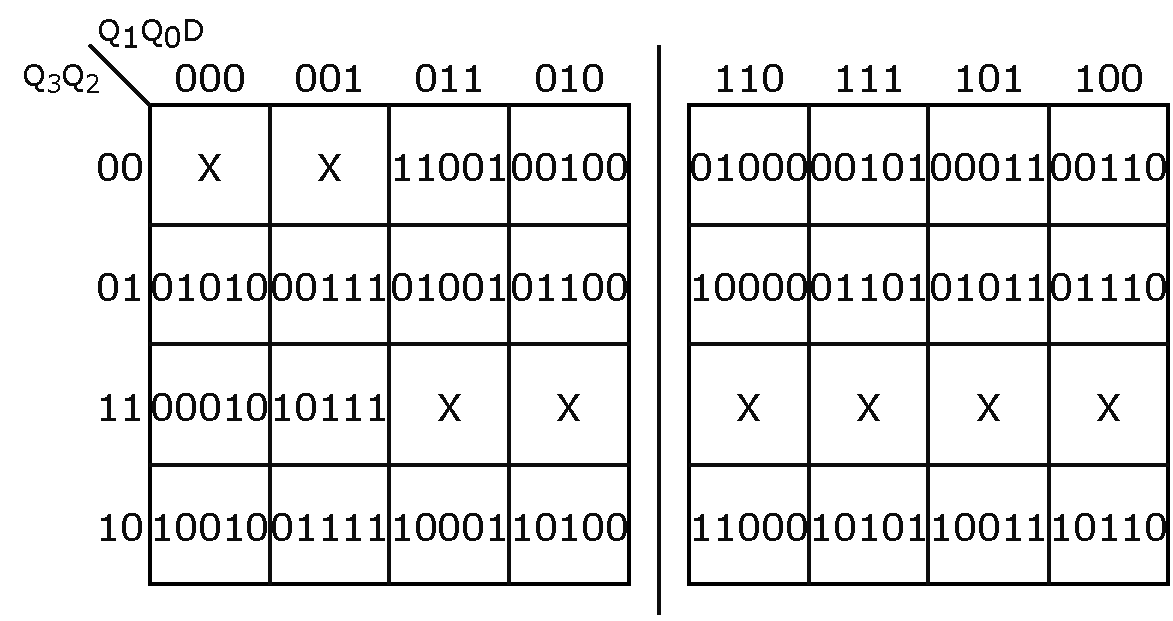
\includegraphics[width=0.6\linewidth]{fig/Karnaugh_12system_2.pdf}
    \end{figure}
    \item 状态方程
    \[\begin{aligned}
    Q_0^{n+1} &= \ol{Q_0}\\
    Q_1^{n+1} &= \ol{Q_1}\ol{Q_0}D+\ol{Q_1}Q_0\ol{D}+Q_1Q_0D+Q_1\ol{Q_0}\ol{D}
                =(Q_0\oplus D)\ol{Q_1}+\ol{Q_0\oplus D}Q_1\\
    Q_2^{n+1} &= \ol{Q_3}Q_2\ol{Q_0}\ol{D}+\ol{Q_2}\ol{Q_1}\ol{Q_0}D+Q_2\ol{Q_1}Q_0+\ol{Q_3}\ol{Q_2}\ol{Q_1}D+Q_2Q_1D+\ol{Q_2}Q_1Q_0\ol{D}\\
    &=(\ol{Q_1}\ol{Q_0}D+Q_1Q_0\ol{D}+\ol{Q_3}\ol{Q_1}D)\ol{Q_2}+(\ol{Q_3}\ol{Q_0}\ol{D}+\ol{Q_1}Q_0+Q_1D)Q_2\\
    Q_3^{n+1} &= Q_3Q_1+\ol{Q_3}Q_2Q_1Q_0\ol{D}+Q_3Q_0+Q_3\ol{Q_2}\ol{Q_1}\ol{D}+Q_3Q_2D+\ol{Q_3}\ol{Q_2}\ol{Q_1}D\\
    &=(Q_2Q_1Q_0\ol{D}+\ol{Q_2}\ol{Q_1}D)\ol{Q_3}+(Q_1+Q_0+\ol{Q_2}\ol{Q_1}\ol{D}+Q_2D)Q_3
    \end{aligned}\]
    \item 驱动方程
    \[\begin{aligned}
    J_0&=1\qquad &K_0&=1\\
    J_1&=Q_0\oplus D \qquad &K_1&=Q_0\oplus D \\
    J_2&=\ol{Q_1}\ol{Q_0}D+Q_1Q_0\ol{D}+\ol{Q_3}\ol{Q_1}D \qquad &K_2&=\ol{\ol{Q_3}\ol{Q_0}\ol{D}+\ol{Q_1}Q_0+Q_1D} \\
    J_3&=Q_2Q_1Q_0\ol{D}+\ol{Q_2}\ol{Q_1}D \qquad &K_3&=\ol{Q_1+Q_0+\ol{Q_2}\ol{Q_1}\ol{D}+Q_2D}
    \end{aligned}\]
\end{enumerate}

\subsection{Protues仿真}
\par 电路图连接如下
\begin{figure}[H]
    \centering
    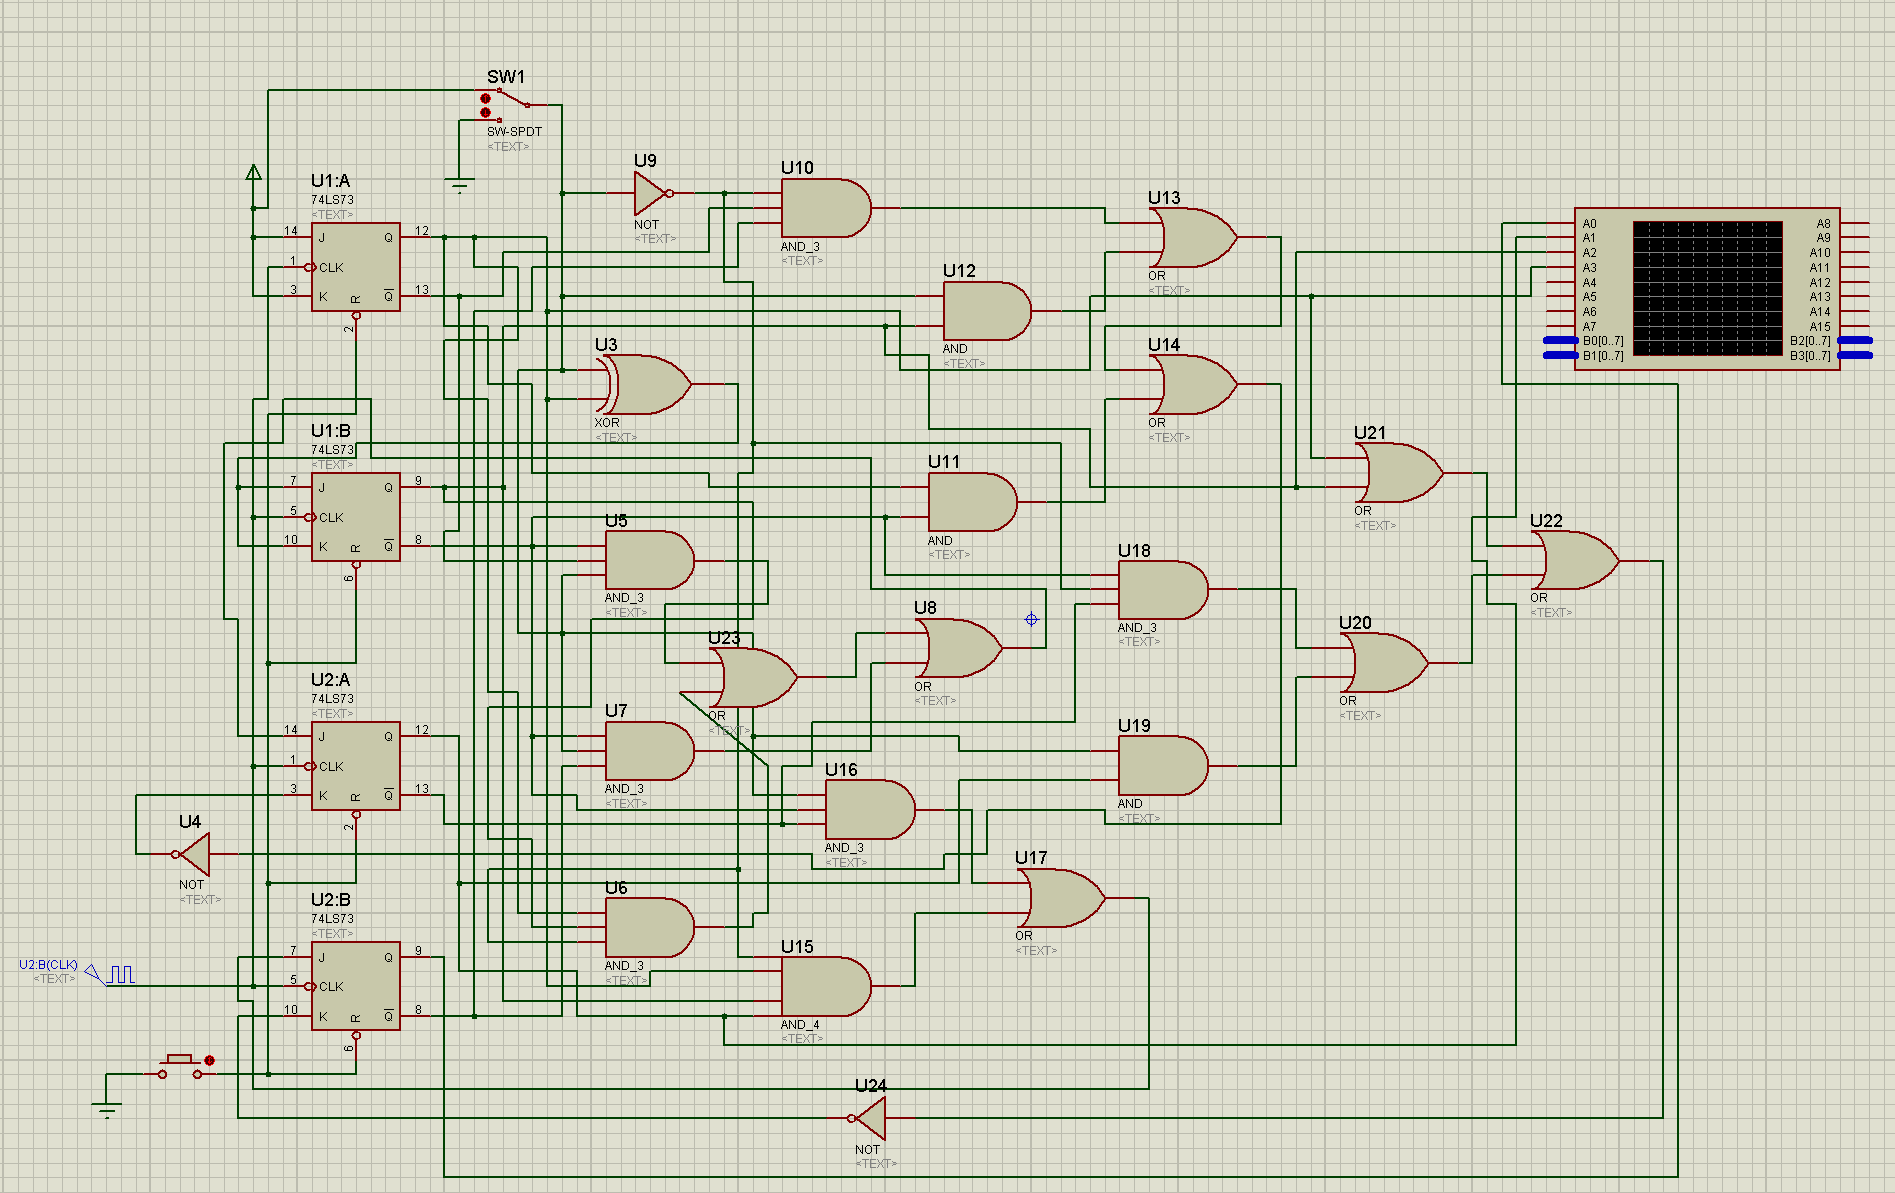
\includegraphics[width=0.8\linewidth]{fig/12system_protues_2.PNG}
\end{figure}
\par 仿真结果如下,正向计数
\begin{figure}[H]
    \centering
    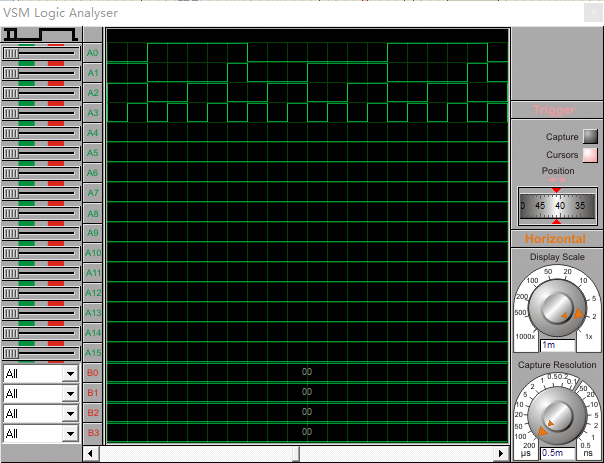
\includegraphics[width=0.6\linewidth]{fig/12system_protues_21.PNG}
\end{figure}
\par 逆向计数
\begin{figure}[H]
    \centering
    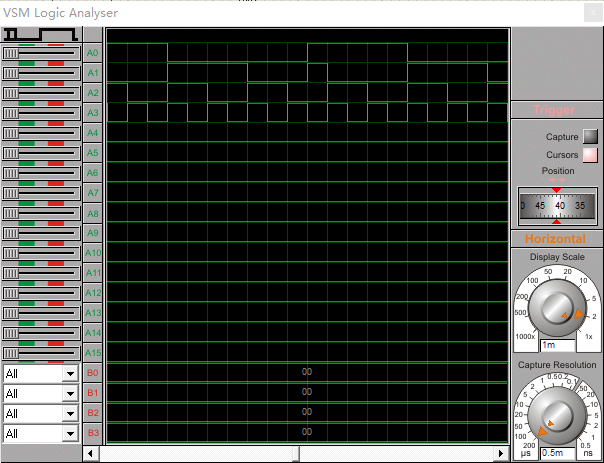
\includegraphics[width=0.6\linewidth]{fig/12system_protues_22.PNG}
\end{figure}
\par 波形符合12进制转换

\subsection{Basys板电路实现}
\par Verilog程序如下,12进制计数器部分,包括控制变量D的实现(变量名为\verb'fb')
\begin{lstlisting}[language=Verilog,basicstyle=\tiny]
module Counter(
    input clr, // clear, say reset
    input wire clk, // clock
    input wire fb, // add or minus
    output [6:0] seg,
    output [3:0] an
    );

    reg [3:0] out;
    parameter MAX_COUNT = 12;
    
    // time counter
    localparam MAX_COUNT_TIME = 50_000_000; // 0.5s
    reg [25:0] count; // 26 bits to store count: 2^26 > 5*10^7
    always @ (posedge clk or posedge clr)
    begin
        if (clr == 1) // reset
            count <= 0;
        else if (count == MAX_COUNT_TIME - 1) // return 0
            count <= 0;
        else
            count <= count + 1;
    end

    // frequency divisor (flip-flop)
    reg clk_div;
    always @ (posedge clk, posedge clr)
    begin
        if (clr == 1)
            clk_div <= 0;
        else if (count == MAX_COUNT_TIME - 1) // reset
            clk_div <= ~clk_div;
        else // set
            clk_div <= clk_div;
    end

    // 12 system counter
    always @ (posedge clk_div or posedge clr)
    if (fb == 0)
        begin
            if (clr == 1)
                out <= 0;
            if (out == MAX_COUNT)
                out <= 0;
            else
                out <= out + 1;
        end
    else
        begin
            if (clr == 1)
                out <= 0;
            if (out == 0)
                out <= 4'b1100;
            else
                out <= out - 1;
        end

    display disp1 (.digit(out),.seven_seg(seg));
    
    // only turn on the first seven segment display
    assign an = 4'b1110;

endmodule
\end{lstlisting}
\par 分频计数器与七段数码管连接部分
\begin{lstlisting}[language=Verilog,basicstyle=\tiny]
\scriptsize
module display (
    input [3:0] digit,
    output reg [6:0] seven_seg
    );

    always @(digit)
        case(digit)
            1: seven_seg = 7'b100_1111;
            2: seven_seg = 7'b001_0010;
            3: seven_seg = 7'b000_0110;
            4: seven_seg = 7'b100_1100;
            5: seven_seg = 7'b010_0100;
            6: seven_seg = 7'b010_0000;
            7: seven_seg = 7'b000_1111;
            8: seven_seg = 7'b000_0000;
            9: seven_seg = 7'b000_0100;
            10: seven_seg = 7'b000_1000; // a
            11: seven_seg = 7'b110_0000; // b
            12: seven_seg = 7'b011_0001; // c
        endcase // clk

endmodule
\end{lstlisting}
\par 限制文件如下
\begin{lstlisting}[language=Verilog,basicstyle=\tiny]
set_property PACKAGE_PIN W4 [get_ports {an[3]}]
set_property PACKAGE_PIN V4 [get_ports {an[2]}]
set_property PACKAGE_PIN U4 [get_ports {an[1]}]
set_property PACKAGE_PIN U2 [get_ports {an[0]}]
set_property PACKAGE_PIN W7 [get_ports {seg[6]}]
set_property PACKAGE_PIN W6 [get_ports {seg[5]}]
set_property PACKAGE_PIN U8 [get_ports {seg[4]}]
set_property PACKAGE_PIN V8 [get_ports {seg[3]}]
set_property PACKAGE_PIN U5 [get_ports {seg[2]}]
set_property PACKAGE_PIN V5 [get_ports {seg[1]}]
set_property PACKAGE_PIN U7 [get_ports {seg[0]}]

set_property PACKAGE_PIN W5 [get_ports clk]
set_property IOSTANDARD LVCMOS33 [get_ports {an[3]}]
set_property IOSTANDARD LVCMOS33 [get_ports {an[2]}]
set_property IOSTANDARD LVCMOS33 [get_ports {an[1]}]
set_property IOSTANDARD LVCMOS33 [get_ports {an[0]}]
set_property IOSTANDARD LVCMOS33 [get_ports {seg[6]}]
set_property IOSTANDARD LVCMOS33 [get_ports {seg[5]}]
set_property IOSTANDARD LVCMOS33 [get_ports {seg[4]}]
set_property IOSTANDARD LVCMOS33 [get_ports {seg[3]}]
set_property IOSTANDARD LVCMOS33 [get_ports {seg[2]}]
set_property IOSTANDARD LVCMOS33 [get_ports {seg[1]}]
set_property IOSTANDARD LVCMOS33 [get_ports {seg[0]}]
set_property IOSTANDARD LVCMOS33 [get_ports clk]

set_property PACKAGE_PIN V17 [get_ports clr]
set_property PACKAGE_PIN R2 [get_ports fb]
set_property IOSTANDARD LVCMOS33 [get_ports clr]
set_property IOSTANDARD LVCMOS33 [get_ports fb]
\end{lstlisting}
\par 最终结果图如下
\begin{figure}[H]
    \centering
    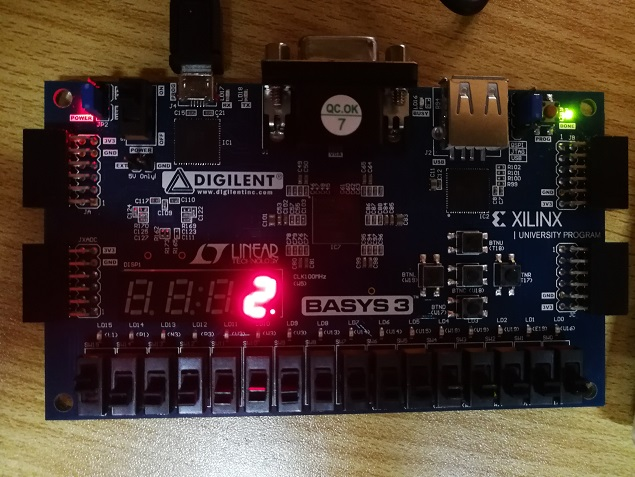
\includegraphics[width=0.6\linewidth]{fig/basys3_12system.jpg}
\end{figure}
\par 通过调整最左下角的拨码开关,可实现任意时刻计数器的正向计数和反向计数


\section{心得体会}
\begin{enumerate}
    \item 学会了移位寄存器及JK触发器的使用及其功能
    \item 明白同步异步时序电路如何进行设计
    \item 更好地学会用Verilog进行电路设计分析,并成功上板实现
\end{enumerate}


\end{document}

%缺检查
%1点阵